
\chapter{Ugeopgave 8-9}
\label{cha:ugeopgave-8-9}

\section{Del 1}
\label{sec:del-1-2}

Emission af fotoner er implementeret i lyskilde-klassen. Her er
pseudokoden fra N4-noten implementeret.

\section{Del 2}
\label{sec:del-2-1}

Fotonspredning (eng: \emph{scattering}) blev implementeret for diffus
reflektion vha. den metode, der er beskrevet i
opgaveformuleringen. Dette sker i \texttt{trace\_photon}-metoden i
\texttt{Surface.cpp}-filen.

\section{Del 3}
\label{sec:del-3-1}

I vores lyskilde-klasse skaleres fotonerne efter udsendelse og
foton-tr�et balanceres derefter.

For at f� skaleringen til at fungere ordentligt �ndrede vi
skaleringsfunktionen i \texttt{Photonmap.cpp}. Oprindeligt udf�rte den
operationen $ photonpower = photonpower * scale $, hvor $scale$ var
$1/antal~af~fotoner$. Med denne operation blev fotonernes \emph{power}
altid sat til $0$. Derfor �ndrede vi skaleringsfunktionen til at
udf�re $photonpower = photonpower / scale$, hvor vi satte $scale$ til
antallet af fotoner i tr�et.

\section{Del 4}
\label{sec:del-4-1}

Et screenshot af vores raytracer, hvor vi har deaktiveret
\emph{ambient}, \emph{lambertian shading} og \emph{phong highlights}
kan ses p� figur \ref{fig:8-4-1}. Vi udsendte $100000$ fotoner og
radius $0.2$ samt $200$ fotoner som argumenter til
\texttt{irradiance\_estimate}-funktionen.

\begin{figure}[htbp]
  \centering
  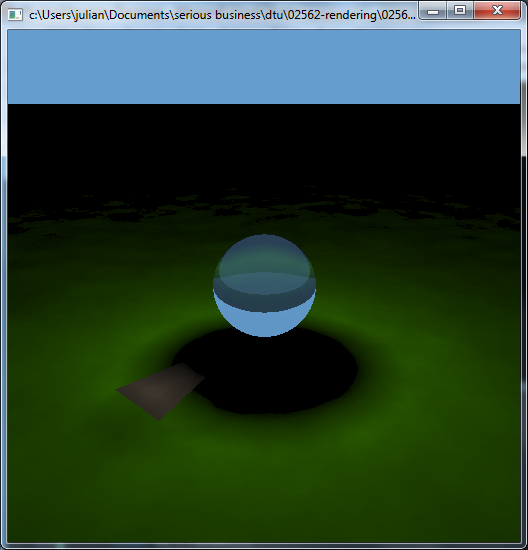
\includegraphics[width=8cm]{screenshots/exc8-9/01_no_caustics_with_specular.png}
  \caption{Diffus reflektion}
  \label{fig:8-4-1}
\end{figure}

\section{Del 5}
\label{sec:del-5-1}

Vi udvidede vores russisk roulette-funktionalitet til ogs� at tage
muligg�re spekul�r reflektion samt refraktion. Til at beregne
fotonernes baner brugte vi samme funktioner som vi udviklede i
forbindelse med den originale raytracer.

Et screenshot af vores raytracer, der nu ogs� kan generere
\emph{caustics} kan ses p� figur \ref{fig:8-5-1}. Vi udsendte $100000$
fotoner og radius $0.2$ samt $200$ fotoner som argumenter til
\texttt{irradiance\_estimate}-funktionen. Ogs� her har deaktiveret
\emph{ambient}, \emph{lambertian shading} og \emph{phong highlights}

\begin{figure}[htbp]
  \centering
  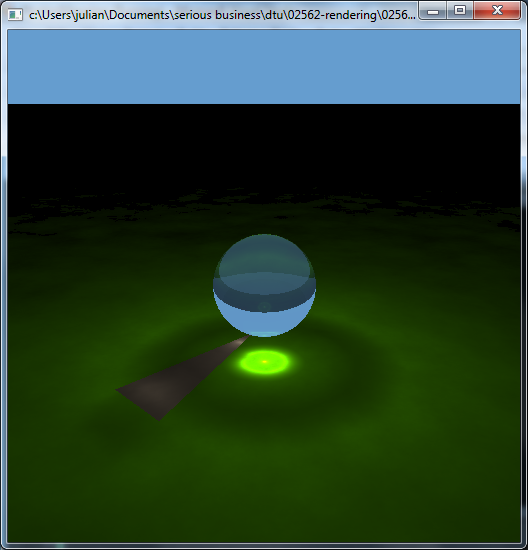
\includegraphics[width=8cm]{screenshots/exc8-9/02-caustics_with_specular.png}
  \caption{Diffus og spekul�r reflektion samt refraktion}
  \label{fig:8-5-1}
\end{figure}

P� figur \ref{fig:8-5-2} ses samme rendering som p� figur
\ref{fig:8-5-1}, blot med lokal belysning aktiveret.

\begin{figure}[htbp]
  \centering
  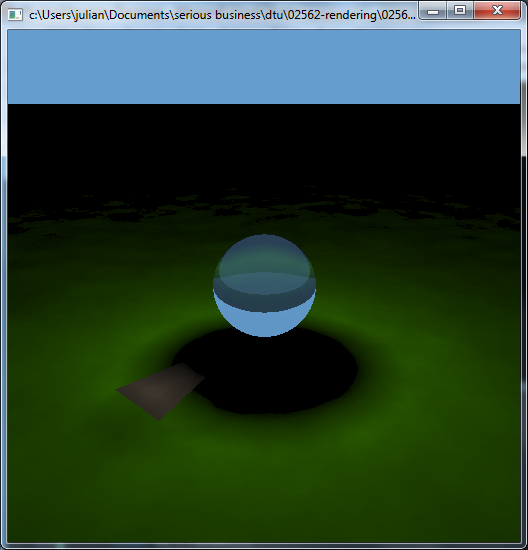
\includegraphics[width=8cm]{screenshots/exc8-9/01_no_caustics_with_specular.png}
  \caption{Diffus og spekul�r reflektion samt refraktion}
  \label{fig:8-5-2}
\end{figure}

%%% Local Variables: 
%%% mode: latex
%%% TeX-master: "report_main"
%%% End: 
